\documentclass[twocolumn,xelatex,ja=standard,jafont=noto]{bxjsarticle}
\usepackage[utf8]{inputenc}

\date{Oct.13 2020}

\usepackage{natbib}
\usepackage{graphicx}
\usepackage{tikz}
\usepackage{circuitikz}
\usepackage{tabularx}
\usepackage{diagbox}
\usepackage{amsmath,amssymb}
\usepackage{hyperref}


\def\ds{\displaystyle}
\def\ul{\underline}
	\title{制御工学3課題1	}
	\author{BQ18026,関宇 }
	\date{Oct.14,2020}
	
	
\begin{document}
		\maketitle
		



\section{次の行列に対する状態遷移行列を計算せよ.また,これらの$ t\to \infty $における極限値と,その行列の固有値の関係について考察せよ.}

状態遷移行列の計算法より,

	\begin{equation}
e^{At}=L^{-1}[(sI-A)^{-1}]
	\end{equation}
	
	1),
	
	\begin{equation}
	    a={
\left[ \begin{array}{cc}
0&0\\
0&0
\end{array}
\right ]}
	\end{equation}
	
	
\begin{equation}
L^{-1}[(sI-A)^{-1}]=L^{-1}[
	    {
\left[ \begin{array}{cc}
\frac{1}{s}&0\\
0&\frac{1}{s}
\end{array}
\right ]}
	]
\end{equation}

\begin{equation}
	    A(a)={
\left[ \begin{array}{cc}
1&0\\
0&1
\end{array}
\right ]}
	\end{equation}
	
	
	2),
	
		\begin{equation}
	    b={
\left[ \begin{array}{cc}
-1&0\\
0&-2
\end{array}
\right ]}
	\end{equation}
	
	
	\begin{equation}
L^{-1}[(sI-A)^{-1}]=L^{-1}[
	    {
\left[ \begin{array}{cc}
\frac{1}{s+1}&0\\
0&\frac{1}{s+2}
\end{array}
\right ]}
	]
\end{equation}

\begin{equation}
	    A(b)={
\left[ \begin{array}{cc}
e^{-t}&0\\
0&e^{-2t}
\end{array}
\right ]}
	\end{equation}
	
	
	3),
	
		\begin{equation}
	    b={
\left[ \begin{array}{cc}
-1&0\\
0&-2
\end{array}
\right ]}
	\end{equation}
	
	
	\begin{equation}
L^{-1}[(sI-A)^{-1}]=L^{-1}[
	    {
\left[ \begin{array}{cc}
\frac{1}{s+1}&0\\
0&\frac{1}{s+2}
\end{array}
\right ]}
	]
\end{equation}

\begin{equation}
	    A(c)={
\left[ \begin{array}{cc}
e^{-t}&0\\
0&e^{-2t}
\end{array}
\right ]}
	\end{equation}
	
	
	4),
	
		\begin{equation}
	    b={
\left[ \begin{array}{cc}
-1&0\\
0&-2
\end{array}
\right ]}
	\end{equation}
	
	
	\begin{equation}
L^{-1}[(sI-A)^{-1}]=L^{-1}[
	    {
\left[ \begin{array}{cc}
\frac{1}{s+1}&0\\
0&\frac{1}{s+2}
\end{array}
\right ]}
	]
\end{equation}

\begin{equation}
	    A(d)={
\left[ \begin{array}{cc}
e^{-t}&0\\
0&e^{-2t}
\end{array}
\right ]}
	\end{equation}
	
	
	5),
	
		\begin{equation}
	    b={
\left[ \begin{array}{cc}
-1&0\\
0&-2
\end{array}
\right ]}
	\end{equation}
	
	
	\begin{equation}
L^{-1}[(sI-A)^{-1}]=L^{-1}[
	    {
\left[ \begin{array}{cc}
\frac{1}{s+1}&0\\
0&\frac{1}{s+2}
\end{array}
\right ]}
	]
\end{equation}

\begin{equation}
	    A(e)={
\left[ \begin{array}{cc}
e^{-t}&0\\
0&e^{-2t}
\end{array}
\right ]}
	\end{equation}
	
	
\section{次のシステムのステップ入力に対する応答 x(t) を求めよ.}

	

(1) DC サーボモータの仕組みについて調べて説明してください(サーボとはどのようなものか,DC モータの構造とエンコーダの仕組みに分けて説明してください).\\

DCモータは,電気的な入力(電流や電圧)によって,機械的な出力,つまり,回転角や回転速度を得るものである.磁界中DCモータの構造は等価回路に置き換えて考えるのが一般的である.

\begin{figure}[h!]
    \centering
    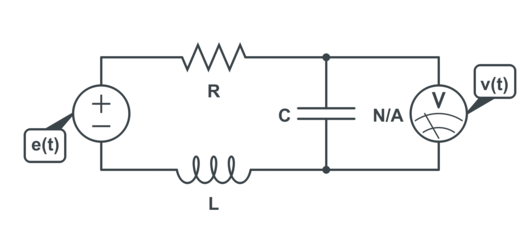
\includegraphics[scale=0.4]{011.png}
    \caption{等価回路 }
\end{figure}

この回路で,Rはモータの電機子抵抗,Lはモータのインダクタンス,Cはコンデンサであり,

固有振動数というのは振動系自身の性質によって特有の振動のことである.例えば外力に加えない時,一回インパルス信号を与えると,振動系が自由振動を行う.この時の振動数は固有振動数である.\\


機械設計する時に事故を防ぐことも重要となってくる.しかし加振力が固有振動数とともに振動する時に共振という現象が発生し,振幅が大きくなって事故が起こしやすいので,これを防ぐために固有振動数を知ることが重要である$ ^{[1]} $.



\section{課題2}

実験で使用するはりの材料はSUS405とSS400の2種類である.それぞれについて,縦弾性係数と密度を調べよ.必ず出典を明記すること$ ^{[6][7]} $.


\begin{table}[!htbp]
\centering
\caption{<金属材料データベース>}
\begin{tabular}{ccc}
\hline
& SUS405 & SS400 \\
\hline
縦弾性係数($ kN/mm^{2} $)& 200& 205\\
密度($ kg/m^{3} $) & 7750& 7850\\
\hline
\end{tabular}
\end{table}



\section{課題3}

図 1 のような幅 b,厚さ h の一様な長方形断面のはりの中立軸 N-N'まわりの断面二次モーメント I を
b と h を用いて表せ.また,断面 2 次モーメントの物理的な意味を説明せよ$ ^{[4]} $.


まず,断面二次モーメントIは定義である(1)式は以下である.


\begin{equation}
			I=\int_{A}^{}y^{2}dA
\end{equation}


ここで,微小面積dAは微小長さdyを用いると,$ dA=bdy $と表せる.さらに積分範囲は中立軸まわりだから,$ -\frac{h}{2}\sim\frac{h}{2} $.これより

\begin{equation}
			I=\int_{-\frac{h}{2}}^{\frac{h}{2}}y^{2}bdy=\frac{bh^{3}}{12}
\end{equation}

断面二次モーメントとは、曲げモーメントに対するはり部材の変形のしにくさを表した量である.


\section{課題4}

\begin{equation}
			F=k\delta
\end{equation}

ばね定数 k を縦弾性係数 E,断面二次モーメント I,はりの長さ L を用いて表せ.




まず先端からの距離Lにおける曲げモーメントM=-FL,これをはりのたわみ方程式に代入して2回微分すればたわみ曲線の方程式が出る.


\begin{equation}
		\frac{d^{2}\delta}{dx^{2}}=-\frac{M}{EI}=\frac{Fx}{EI}
\end{equation}

1回目

\begin{equation}
		\frac{d\delta}{dx}=\int\frac{Fx}{EI}dx=\frac{F}{2EI}x^{2}+C_{1}
\end{equation}

続いて2回目の積分


\begin{equation}
		\delta=\int(\frac{F}{2EI}x^{2}+C_{1})dx=\frac{F}{6EI}+C_{1}x+C_{2}
\end{equation}

これを求めるには積分定数の$ C_{1},C_{2} $を境界条件から決める.また,最大たわみははりの先端,すなわち$ x=0 $で生じるから,

\begin{equation}
	\delta=\frac{FL^{3}}{3EI}
\end{equation}


$ F=k\delta $から,$ k=\frac{F}{\delta} $.よって,



\begin{equation}
	k=\frac{3EI}{L^{3}}
\end{equation}





\section{課題5}
はりの横振動の運動方程式を導出せよ$ ^{[2]} $.

\begin{equation}
			\frac{\partial^{2}}{\partial x^{2}}[EI\frac{\partial^{2}y}{\partial x^{2}}]+\rho A\frac{\partial^{2}y}{\partial t^{2}}=0
\end{equation}


ニュートンの方程式$ F=ma $より,微小要素y方向の運動方程式は,

\begin{equation}
			(\rho Adx)\frac{\partial^{2}y(x,t)}{\partial t^{2}}=Q+\frac{\partial Q}{\partial x}dx-Q=\frac{\partial Q}{\partial x}dx
\end{equation}

となる.そしてせん断力$ Q(x,t) $をたわみ$ y(x,t) $であらわすため,まず座標$ x+dx $の位置に関するモーメントのつり合いを考えると,


\begin{equation}
			M(x,t)+\frac{\partial M(x,t)}{\partial x}dx-M(x,t)+Q(x,t)dx=0
\end{equation}

となり,次式を得る.


\begin{equation}
			\frac{\partial M(x,t)}{\partial x}d=-Q(x,t)
\end{equation}


材料力学の知識より,曲げモーメントとそれによって生じる変位との関係は次式で与えられる.


\begin{equation}
			EI(x)\frac{{\partial^{2}y(x,t)}}{\partial x^{2}}=M(x,t)
\end{equation}


式を代入すると次式を得る


\begin{equation}
			\rho A(x)\frac{\partial^{2}y(x,t)}{\partial t^{2}}+\frac{\partial^{2}}{\partial x^{2}} (EI(x)\frac{\partial^{2}y(x,t)}{\partial x^{2}})=0
\end{equation}


これがはりの運動方程式である.とくに,はりが均質で一様な断面を持つ場合は,$ EI(x),A(x) $は一定であるので,上式は以下のようになる.


\begin{equation}
			\rho A\frac{\partial^{2}y(x,t)}{\partial t^{2}}+EI\frac{\partial^{4}y(x,t)}{\partial x^{4}}=0
\end{equation}


\newpage



\section{課題6}
片持ちばりの横振動の境界条件として自由端において次の関係を与える$ ^{[3]} $.



\begin{equation}
			\frac{\partial^{2}y}{\partial x^{2}}=0, \frac{\partial^{3}y}{\partial x^{3}}=0
\end{equation}\\


自由端の境界条件がこのように表される理由を説明せよ.\\


境界条件としては,自由端の曲げモーメントは0である.よって,



\begin{equation}
			 \frac{\partial^{2}y}{\partial x^{2}}=0
\end{equation}


そしてせん断力も0である.式

\begin{equation}
			 \frac{\partial M(x,t)}{\partial x}d=-Q(x,t)
\end{equation}

より,せん断力は

\begin{equation}
			Q(x,t)=-EI(x)\frac{\partial^{3}y}{\partial x^{3}}
\end{equation}


つまり


\begin{equation}
			 \frac{\partial^{3}y}{\partial x^{3}}=0
\end{equation}





\newpage


\section{}
\begin{thebibliography}{9}
\bibitem{latexcompanion} 
岩壺 卓三,松久 寛, 井上喜雄, 宇津野秀夫, 河村庄造, 神吉博, 小泉孝之, 塩幡宏規  
[\textit{振動工学の基礎}]. 
 (2019/2/20),   p.5.116.117.118 森北出版株式会社

\bibitem{latexcompanion} 
沢 俊行 
[\textit{再入門・材料力学 基礎編}]. 
(2007/10/22),   p.107.133 ものづくりの教科書


\bibitem{einstein} 
ステンレス協会
[\textit{ステンレスのヤング率、ポアソン比など機械的性質について}]. 
\url{http://www.jssa.gr.jp/contents/faq-article/q6/}


\bibitem{einstein} 
ステンレス協会
[\textit{主な機械材料の物理的性質}]. 
\url{http://www.me.cit.nihon-u.ac.jp/lab/ben/LectureCourse/New_1Mechanics/Material_Properties.pdf}



\end{thebibliography}





\end{document}